% SHG FROG 及 PCGPA

如果我们要测量线偏振的超快激光脉冲的波形(即电场关于时间的函数), 我们不能直接用仪器测量, 因为电子元件的时间分辨率远远不够. 但我们可以使用 Frequency Resolved Optical Gating (FROG). FROG 有许多不同的实现方法, 这里只讨论比较常见的 SHG FROG(Second Harmonic Generation FROG) 和 \bb{PCGPA}.

\begin{figure}[ht]
\centering
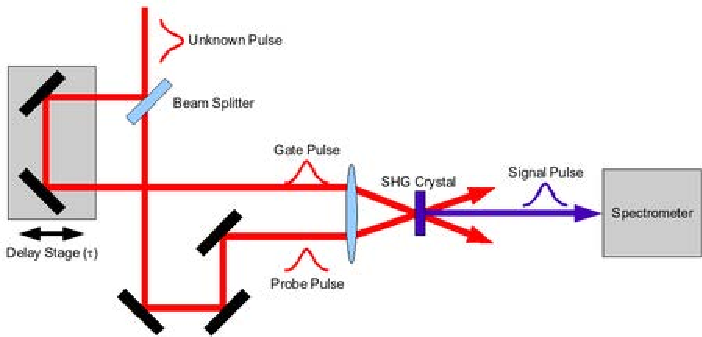
\includegraphics[width=12cm]{./figures/Frog1.pdf}
\caption{SHG FROG 的光路(图片来自 WikiPedia)} \label{Frog_fig1}
\end{figure}

\begin{figure}[ht]
\centering
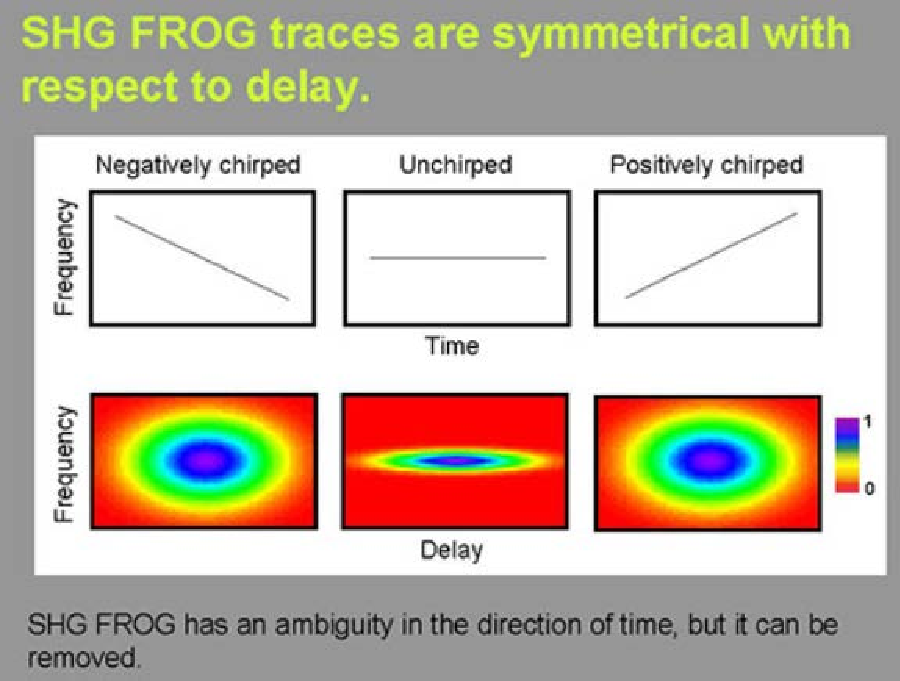
\includegraphics[width=10cm]{./figures/Frog2.pdf}
\caption{SHG FROG trace(图片来自网络)} \label{Frog_fig2}
\end{figure}

Frog 的大概原理就是把被测量的脉冲(prob) $f(t)$ 和另一个脉冲(gate) $g(t)$ 叠加(注意 $f(t)$ 和 $g(t)$ 都是实函数), 然后通过一个二阶非线性介质产生一个 $f(t)g(t)$ 脉冲并分离出来, 再测量光谱(即傅里叶变换). 接下来我们可以控制两个脉冲的相对延迟(time delay) $\tau$, 就得到不同延迟下 $f(t - \tau)g(t)$ 的光谱, 也就是一个二维函数, 叫做 \bb{FROG trace}(\autoref{Frog_fig2}). 很多情况下, gate 就是 prob 通过一个 beam splitter 分出来的, 实验光路如\autoref{Frog_fig1} 所示.% 有一个问题, 就是光谱仪可以得到负频率的光谱吗

% 未完成: 是否可以讲讲 SLM 全息的 GS 算法
\begin{equation}\label{Frog_eq1}
a(\omega, \tau) = \abs{\int_{-\infty}^{\infty} f(t-\tau) g(t) \E^{-\I\omega t} \dd{t}}^2
\end{equation}
只要用特定的算法, 就可以从\autoref{Frog_eq1} 中解出 $f(t)$ 和 $g(t)$.

\subsection{PCGPA 算法}

PCGPA(Principal Component General Projection Algorithm)就是从\autoref{Frog_eq1} 中解出 $f(t)$ 和 $g(t)$ 的一种常见算法. 在得到 我们假设 $f(t)$ 和 $g(t)$ 都是等时间间隔的离散点 $f_1, f_2\dots, f_N$ 和 $g_2, g_2\dots, g_N$, 可以看成两个列矢量. 我们先来做两矢量的外积, 即

\begin{equation}
\vec f \vec g\Tr = \pmat{
f_1g_1 & \ldots & f_1g_N\\
\vdots & \ddots & \vdots\\
f_Ng_1 & \ldots & f_Ng_N}
\end{equation}
然后我们把第 $i$ 行向左移动 $i-1$ 个元(左边多出的矩阵元补到右边), 得到
\begin{equation}
\pmat{
f_1g_1 & f_1g_2 & \ldots & f_1g_N\\
f_2g_2 & f_2g_3 & \ldots & f_2g_1\\
\vdots & \vdots & \vdots & \vdots\\
f_Ng_N & f_Ng_1 & \ldots & f_Ng_{N-1}
}\end{equation}
现在可以发现每一列恰好是 $f(t-\tau)g(t)$ 的离散形式\footnote{唯一的区别是从最上面移出的 $g_i$ 跑到了最下面, 而在实验中最下面应该由 0 来填补. 但如果 $\vec f$ 和 $\vec g$ 矢量的首尾都有足够多的 0, 这个问题就自动解决了.}, 第 $i$ 列 $\tau = (i - 1)\Delta t$. 然而当 $i > N/2$ 的时候, 更自然的理解是  $\tau = (i-N)\Delta t$. 例如与其认为第 $N$ 列是 $g$ 向上移动了 $N-1$ 个元, 倒不如认为是向下移动了 $1$ 个元. 根据这种思想, 我们可以把矩阵左半和右半调换得到
\begin{equation}
\pmat{
f_1g_{N/2 + 1} & f_1g_{N/2+2} & \ldots  & f_1g_{N/2}\\
f_2g_{N/2 + 2} & f_2g_{N/2+3} & \ldots  & f_2g_{N/2+1}\\
\vdots               & \vdots               & \vdots & \vdots\\
f_Ng_{N/2}       & f_Ng_{N/2+1}   & \ldots   & f_Ng_{N/2-1}
}\end{equation}
这样, 从左到右的每列分别对应从 $\tau = -(N/2)\Delta t, \dots, (N/2 - 1)\Delta t$.

现在我们对每一列做离散傅里叶变换(注意前后都要 fftshift), 就得到了含相位的 Frog trace 矩阵, 其中的每一列都是\autoref{Frog_eq1} 中的
\begin{equation}
\int_{-\infty}^{\infty} f(t-\tau) g(t) \E^{-\I\omega t} \dd{t}
\end{equation}


% 未完成: 这里有一个问题就是公式中是 f(t-\tau)g(t), 而矩阵中却是 f(t)g(t+\tau) 啊.
